\documentclass{standalone}

\usepackage{tikz}
\usetikzlibrary{shapes.geometric}

\begin{document}

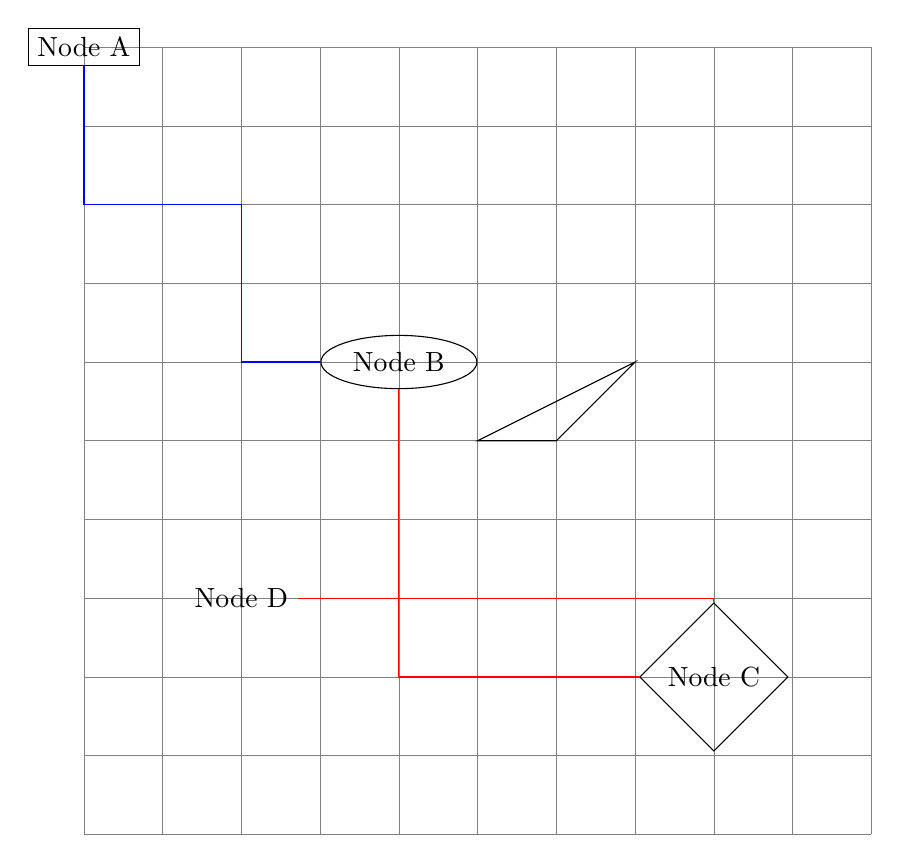
\begin{tikzpicture}

\draw [help lines] (-5,-5) grid (5,5);

\draw (0,0) -- (1,0) -- (2,1) -- cycle;

\path node [draw] (A) at (-5,5) {Node A};
\path node [draw,ellipse] (B) at (-1,1) {Node B};

\path node [draw,diamond] (C) at (3,-3) {Node C};

\draw node (D) at (-3,-2) {Node D};

\draw [color=blue] (node cs:name=A,anchor=south) |- (-3,3) |- (node cs:name=B,anchor=west);
\draw [color=red] (node cs:name=B,anchor=south) |- (node cs:name=C,anchor=west);

\draw [color=red] (node cs:name=C,anchor=north) |- (node cs:name=D,anchor=east);

\end{tikzpicture}

\end{document}